% =====================================================================
%  Riwayah-aware automatic recognition of Quranic Tajweed rules
%  Springer LNCS (llncs.cls v2.24) conference manuscript
%
%  Compile with:  pdflatex paper && bibtex paper && pdflatex paper && pdflatex paper
%  Page limit: 20 pages including references, tables and figures.
% =====================================================================
\documentclass[runningheads]{llncs}

\usepackage{amsmath,amssymb}
\usepackage{graphicx}
\usepackage{xcolor}
\usepackage{url}
\usepackage{microtype}

% Editorial markers for details that must be supplied by the authors
% before submission (see OPEN_ITEMS.md).  Remove the redefinition of
% \todo{} once every marker has been resolved.
\newcommand{\todo}[1]{\textcolor{red}{\textbf{[TODO: #1]}}}

\graphicspath{{figures/}}

\begin{document}

\title{Automatic Recognition of Quranic Tajweed Rules Across Riwayat:
A Corpus and Machine-Learning Study of Idgham and Qalqalah\todo{confirm final title}}
\titlerunning{Automatic Recognition of Quranic Tajweed Rules Across Riwayat}

\author{First Author\inst{1}\orcidID{0000-0000-0000-0000} \and
Second Author\inst{2}\orcidID{0000-0000-0000-0000}}
\authorrunning{F. Author and S. Author}
\institute{First Affiliation, City, Country \and
Second Affiliation, City, Country\\
\email{first.author@example.org, second.author@example.org}
\todo{replace author block, affiliations and ORCIDs}}

\maketitle

\begin{abstract}
Automatic assessment of Quranic recitation requires systems that determine not
only \emph{what} was recited but \emph{how} it was pronounced. We present a
riwayah-aware framework for the automatic recognition of Tajweed rules from
speech. A corpus of 7{,}998 verse-level recordings (11.17\,h) was built from
MP3Quran recitations of Juz' 'Amma by fifteen reciters covering the riwayat of
Hafs 'an 'Asim, Warsh 'an Nafi', and Qalun 'an Nafi'; verse segments were
obtained by forced alignment with manual reconciliation, and occurrences of
Idgham and Qalqalah were localised through rule-based candidate extraction,
manual acoustic annotation and expert verification (705 unique textual
occurrences). Recitation segments are described by eight interpretable acoustic
descriptors and classified into five Tajweed categories with SVM, random
forest, $k$-nearest neighbours, XGBoost and a multilayer perceptron. The
proposed representation outperforms an MFCC baseline with deltas for every
classifier, reaching a Macro-F1 of 0.6935 with XGBoost and gains of up to
$+0.1348$. Ablation identifies duration and a depth metric as the dominant
cues, SMOTE raises Idgham bila-Ghunnah recall from 0.0678 to 0.4915, and
cross-riwayah transfer yields Macro-F1 values of 0.6584--0.6718.

\keywords{Quranic recitation \and Tajweed recognition \and Idgham \and
Qalqalah \and acoustic feature extraction \and machine learning \and
riwayah-aware classification}
\end{abstract}


% =====================================================================
\section{Introduction}
\label{sec:intro}

Qur'anic recitation is a highly structured form of oral Arabic whose
pronunciation is governed by the principles of Tajweed and normally acquired
through repeated practice with expert feedback. Conventional assessment
therefore depends on expert listening, making frequent, scalable and objective
evaluation difficult outside formal instruction. Recitation is further
transmitted through recognised \emph{riwayat}---narrations sharing the same
Qur'anic text but differing in phonetic, articulatory and recitational
detail---so a computational system must treat legitimate riwayah variation as
distinct from pronunciation error. This study considers the ``Big Three''
riwayat: Hafs 'an 'Asim, Warsh 'an Nafi', and Qalun 'an Nafi'.

Automatic assessment of Qur'anic recitation differs fundamentally from
conventional speech recognition, which determines what was recited rather than
how particular phonetic sequences were realised; reciter identification models
speaker characteristics, and generic pronunciation assessment provides no
explicit rule-level representations. The central challenge is thus to detect
specific Tajweed phenomena from the acoustic signal despite speaker variability,
riwayah-related differences and scarce annotated resources---a challenge for
which appropriately annotated speech data is a prerequisite that existing
Qur'anic corpora do not meet (Sect.~\ref{sec:related}).

Idgham and Qalqalah offer complementary test cases. Idgham is an assimilation
between adjacent consonants that modifies the temporal and spectral structure
of the affected boundary, optionally with nasalisation (ghunnah); Qalqalah is an
echo-like release of the consonants \emph{qaf, ta', ba', jim, dal} in sukun
states. Their contrasting signatures make them suitable for testing whether
conventional acoustic descriptors capture rule-specific information while
remaining robust across riwayat.

Prior work leaves four aspects insufficiently explored: the dominance of
lexical- and speaker-level objectives over explicit Tajweed modelling; the
scarcity of studies treating a rule occurrence---rather than an utterance---as
the unit of analysis; the absence of rule-level temporal annotations; and the
unexamined influence of multiple riwayat on acoustic realisation and detection.
This paper therefore treats corpus construction, riwayah identification,
rule-level annotation, feature extraction, supervised classification and
evaluation as interconnected components of one problem.

The contributions are fourfold. \emph{Resource}: a Qur'anic speech corpus
covering the Big Three riwayat, annotated at the Tajweed-rule level.
\emph{Method}: a riwayah-aware pipeline connecting annotation with acoustic
feature extraction and supervised classification. \emph{Experimental}: a
quantitative evaluation of five classifiers on Idgham and Qalqalah across the
three riwayat. \emph{Application}: a foundation for computer-assisted
recitation systems providing rule-specific, interpretable feedback while
respecting legitimate riwayah variation.


% =====================================================================
\section{Related Work}
\label{sec:related}

\subsection{Qur'anic Speech Resources and Recognition}

Existing Qur'anic speech resources differ considerably in scale, speaker
diversity, recording conditions, annotation granularity and intended use
(Table~\ref{tab:corpora}). Verse-level repositories such as
EveryAyah~\cite{everyayah} link recordings to verses but provide no temporal
Tajweed annotation, and the large-scale ASR corpora---the 581{,}216-recording
Quran Recitations corpus~\cite{quran_recitations_asr} and the speaker-disjoint
Quran-Ayah-Corpus~\cite{quran_ayah_corpus}---prioritise transcription over
pronunciation correctness. Diversity-oriented resources
(Tarteel~\cite{khan2023tarteel}, Ar-DAD~\cite{ardad}, QDAT~\cite{qdat} and the
crowdsourced corpus of non-Arabic-speaking reciters~\cite{quranic_audio_crowd})
contribute speakers, realistic conditions or expert judgements, but only text-
or category-level supervision. Transmission-aware resources are the most recent
step: AQQD~\cite{smail2024aqqd} adds qira'at and phonetic-variation metadata and
Riwaya-ID~\cite{riwaya_id} separates Warsh from Hafs with 82\% accuracy using
wav2vec~2.0~\cite{baevski2020wav2vec} and Whisper~\cite{radford2023whisper}, yet
neither provides temporally localised rule labels. Collectively these resources
trade lexical and speaker coverage against rule-level supervision, so corpus
size alone cannot satisfy the requirements of automatic Tajweed recognition.

\begin{table}[t]
\centering
\caption{Comparison of Qur'anic speech resources. ``Rule-level temporal
labels'' indicates whether the resource localises individual Tajweed
phenomena in time.}
\label{tab:corpora}
\begin{tabular}{lllll}
\hline
Resource & Recordings & Speakers & Supervision & Rule-level \
\hline
EveryAyah~\cite{everyayah} & verse-level & professional & verse--audio link & no \
Tarteel~\cite{khan2023tarteel} & $\approx$25{,}000 (67.39\,h) & $>$1{,}200 & audio--text & no \
Ar-DAD~\cite{ardad} & 15{,}810 $+$ 397 & 30 $+$ 12 & reciter identity & no \
QDAT~\cite{qdat} & $>$1{,}500 & $>$150 & 3 rules, expert & categorical \
Crowdsourced~\cite{quranic_audio_crowd} & $\approx$7{,}000 (1{,}166 ann.) & 1{,}287 & 6 categories & categorical \
Quran Recitations~\cite{quran_recitations_asr} & 581{,}216 ($\approx$2{,}882\,h) & 44 & transcript & no \
Quran-Ayah-Corpus~\cite{quran_ayah_corpus} & 263{,}263 & 44 & transcript, disjoint splits & no \
AQQD~\cite{smail2024aqqd} & 24{,}183 & 309 & qira'at metadata & partial \
Riwaya-ID~\cite{riwaya_id} & $>$700\,h & -- & riwayah label (82\%) & no \
Ours & 7{,}998 (11.17\,h) & 15 & rule-level, expert-verified & yes \
\hline
\end{tabular}
\end{table}

\subsection{Automatic Tajweed Recognition}

Acoustic Tajweed assessment began with phoneme-duration analysis of Madd and
Ghunnah~\cite{mohammed2018madd} and progressed through MFCC-based statistical
and neural classifiers for Qalqalah~\cite{qalqalah_vq,qalqalah_mlp}, binary SVM
formulations~\cite{alagrami2021smartajweed}, convolutional~\cite{omran2023cnn}
and recurrent~\cite{alahjal2023lstm} models, and hybrid ASR--classification
pipelines~\cite{tajweedai} (Table~\ref{tab:systems}). Three conclusions recur
across these settings: Tajweed phenomena are not equally separable acoustically;
accuracy alone is insufficient under class imbalance; and performance obtained
under controlled conditions does not imply robust generalisation to unseen
speakers, recordings or riwayat. Idgham and Qalqalah nonetheless remain
fragmented across datasets, feature representations and evaluation protocols,
with no unified framework spanning multiple reciters and transmission
traditions.

\begin{table}[t]
\centering
\caption{Prior automatic Tajweed recognition systems compared with the present
study. Acc.\ = accuracy; val.\ = validation.}
\label{tab:systems}
\begin{tabular}{llllll}
\hline
Study & Rules & Representation & Model & Data & Reported result \
\hline
Mohammed et al.~\cite{mohammed2018madd} & Madd, Ghunnah & duration & threshold & 10 reciters & interpretable cues \
Qalqalah VQ~\cite{qalqalah_vq} & Qalqalah & MFCC & vector quant. & -- & feasibility \
Qalqalah MLP~\cite{qalqalah_mlp} & Qalqalah Kubra & MFCC & MLP & -- & feasibility \
Smartajweed~\cite{alagrami2021smartajweed} & 4 binary rules & filter bank & RBF-SVM & -- & 99\% val.\ acc. \
Omran et al.~\cite{omran2023cnn} & Qalqalah & MFCC & CNN & 3{,}322 / 4 rec. & 90.8\% val.\ acc. \
Al-ahjal et al.~\cite{alahjal2023lstm} & 3 rules & MFCC & LSTM & $>$1{,}500 (QDAT) & 77.0/59.4/66.1\% \
TajweedAI~\cite{tajweedai} & Qalqalah & ASR $+$ alignment & hybrid & internal/ext. & 100\% / 57.14\% \
Ours & 2 Idgham $+$ 3 Qalqalah & 8 descriptors & 5 classifiers & 7{,}998 / 15 rec. & Macro-F1 0.6935 \
\hline
\end{tabular}
\end{table}

\subsection{Research Gap and Positioning}

Four gaps define the present work. First, large ASR corpora provide verse-level
textual supervision whose objective---transcription---does not encode whether a
rule was correctly realised. Second, rule-level temporal annotation identifying
\emph{where} a phenomenon occurs in continuous recitation is largely absent,
preventing models from learning rule realisations independently of context.
Third, rule-specific datasets trade speaker diversity against acoustic control:
four professional reciters~\cite{omran2023cnn} versus crowdsourced but
heterogeneous recordings~\cite{qdat}. Fourth, riwayah is treated as a global
classification target~\cite{riwaya_id} rather than as a factor shifting the
acoustic realisation of individual rules. The proposed study addresses these
gaps by formulating Idgham and Qalqalah recognition as a riwayah-aware,
fine-grained acoustic learning problem on a rule-annotated corpus that retains
reciter and riwayah identity, bridging large-scale Qur'anic ASR research and
rule-specific Tajweed assessment.


% =====================================================================
\section{Methodology}
\label{sec:methodology}

The framework treats automatic Tajweed recognition as a sequence of dependent
stages (Fig.~\ref{fig:framework}). Full-surah recordings are aligned and
segmented into verse-level clips with explicit reciter and riwayah metadata
(Sect.~\ref{sec:corpus}); Tajweed occurrences are localised acoustically through
a hybrid rule-based, expert-verified annotation protocol
(Sect.~\ref{sec:annotation}); segments are represented by interpretable acoustic
descriptors and analysed for redundancy and imbalance
(Sect.~\ref{sec:analysis}); and the resulting instances support a five-class
supervised task evaluated with complementary classifiers, ablations, balancing
strategies, an MFCC baseline, cross-riwayah transfer and bootstrap uncertainty
estimation (Sects.~\ref{sec:ml}--\ref{sec:results}). Three principles govern the
pipeline: the rule occurrence, not the verse, is the unit of analysis; riwayah
identity is preserved at every stage so that legitimate variation can be
separated from error; and every derived artefact remains linked to the original
signal and to the canonical text.

\begin{figure}[t]
\centering
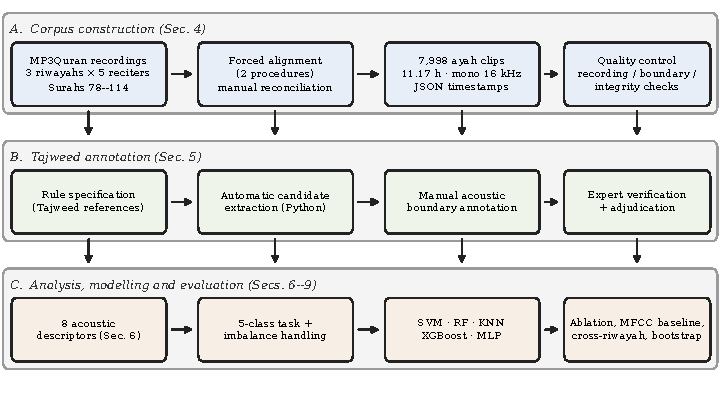
\includegraphics[width=\textwidth]{fig1_framework.pdf}
\caption{Overview of the riwayah-aware Tajweed recognition framework: corpus
construction with forced alignment and quality control (Sect.~\ref{sec:corpus}),
hybrid Tajweed annotation (Sect.~\ref{sec:annotation}), and acoustic analysis,
modelling and evaluation (Sects.~\ref{sec:analysis}--\ref{sec:results}).}
\label{fig:framework}
\end{figure}


% =====================================================================
\section{Corpus Construction}
\label{sec:corpus}

\subsection{Source Material and Riwayah Coverage}

Audio was collected from the publicly available MP3Quran repository of complete
Qur'anic recitations~\cite{mp3quran}. Rather than restricting the corpus to one
tradition, three riwayat were included---Hafs 'an 'Asim, Warsh 'an Nafi', and
Qalun 'an Nafi'---each represented by five reciters, giving fifteen reciters in
total. Reciter selection prioritised inter-speaker variability (vocal
characteristics, articulation, rate, prosody) within a well-defined tradition,
because a model trained on a single reciter may learn speaker-specific rather
than rule-specific characteristics. The scope is Juz' 'Amma (surahs 78--114),
i.e.\ 37 surahs and 564 ayat per reciter, targeting 555 full-surah recordings;
the canonical content corresponds to 8{,}460 reciter--ayah instances, of which
approximately 14.14\,h of full-surah audio were collected.

\subsection{Segmentation, Alignment and Quality Control}

Complete surah recordings were processed with two automatic forced-alignment
procedures whose timestamps and recognised text were retained separately and
reconciled manually into a consolidated segmentation file per surah, from which
ayah-level clips were extracted; this prevents alignment or recognition errors
from propagating unchecked into the training data. Quality control operated at
three levels: recording level (availability, readability, correspondence with
the intended surah and reciter); segmentation level (cross-method comparison and
review of boundaries); and data-integrity level (expected surah and ayah counts
checked against the canonical structure, with missing recordings identified
explicitly rather than treated as complete). Alignment confidence scores are
stored to flag potentially unreliable segments.

\subsection{Corpus Organisation and Statistics}

The corpus separates original recordings from derived segments and metadata:
per-riwayah directories contain, for each reciter, an \texttt{audio/} folder of
full-surah recordings, an \texttt{ayat/} folder of verse segments, and JSON
timestamp files linking every segment to its source position. After
segmentation, alignment and validation, 7{,}998 verse-level recordings were
retained---94.5\% of the theoretical maximum---comprising 11.17\,h of aligned
audio distributed evenly across riwayat (Table~\ref{tab:corpus}); for modelling,
audio is decoded to mono at 16\,kHz. The longer mean verse duration of Warsh and
Qalun relative to Hafs is consistent with differences in recitation tempo and in
the realisation of prolongation (madd) rules.

\begin{table}[t]
\centering
\caption{Composition of the verse-level corpus by riwayah.}
\label{tab:corpus}
\begin{tabular}{lrrrr}
\hline
Riwayah & Reciters & Recordings & Duration (h) & Mean verse dur.\ (s) \\
\hline
Hafs 'an 'Asim  & 5 & 2{,}739 & 3.57 & 4.69 \\
Warsh 'an Nafi' & 5 & 2{,}562 & 3.78 & 5.30 \\
Qalun 'an Nafi' & 5 & 2{,}697 & 3.83 & 5.11 \\
\hline
Total           & 15 & 7{,}998 & 11.17 & 5.03 \\
\hline
\end{tabular}
\end{table}

Rule extraction from the canonical text identified 328 Idgham and 377 Qalqalah
occurrences within Juz' 'Amma---705 unique textual occurrences before
replication across reciters and riwayat (Table~\ref{tab:occurrences}). Because
each occurrence is realised by up to fifteen reciters, the number of acoustic
instances available for learning is substantially larger than the textual
counts, enabling the same phenomenon to be studied under diverse speakers and
riwayat. Recording duration is balanced across riwayat (32--34\% each), whereas
subtype frequencies are strongly skewed: Lam Shamsiyyah accounts for more than
72\% of Idgham occurrences while Idgham Lam-Ra occurs once, and Qalqalah Kubra
(12 occurrences) is far rarer than Qalqalah Wusta (145).

\begin{table}[t]
\centering
\caption{Unique textual occurrences of the annotated Tajweed subtypes in Juz'
'Amma. Subtypes marked $\dagger$ constitute the five-class recognition task of
Sect.~\ref{sec:ml}; the remainder are annotated but excluded from the present
classification experiments\todo{confirm subtype-exclusion criteria}.}
\label{tab:occurrences}
\begin{tabular}{lrlr}
\hline
Idgham subtype & Occ. & Qalqalah subtype & Occ. \\
\hline
Lam Shamsiyyah & 237 & Qalqalah Wusta$^\dagger$       & 145 \\
Idgham bi-Ghunnah$^\dagger$ & 65 & Qalqalah Sughra$^\dagger$      & 123 \\
Idgham bila-Ghunnah$^\dagger$ & 25 & Qalqalah Mushaddadah$^\dagger$ & 97 \\
Idgham Lam-Ra & 1 & Qalqalah Kubra & 12 \\
\hline
Total & 328 & Total & 377 \\
\hline
\end{tabular}
\end{table}


% =====================================================================
\section{Annotation Methodology}
\label{sec:annotation}

Annotation provides rule-specific labels at the level of individual ayat. The
protocol derives from established Tajweed references, whose linguistic and
phonetic descriptions were translated into explicit, consistently applicable
annotation criteria, and combines automatic candidate identification with manual
acoustic verification and expert review.

\subsection{Idgham}

Idgham denotes the assimilation of one consonant into a following consonant,
here primarily nun sakinah and tanwin before the letters designated for Idgham,
optionally with nasalisation. Acoustically it is expected to remove or reduce an
independent realisation of the first consonant, increase temporal overlap
between adjacent segments, and yield a boundary dominated by the following
consonant, with added low-frequency energy and nasal resonance when ghunnah is
present. Candidates were extracted from the Qur'anic text by a Python script
encoding the formal Tajweed conditions; the waveform and spectral representation
of each corresponding recording were then inspected to localise the realisation
and confirm the assimilation. Boundaries were placed to capture the acoustic
event while excluding unrelated segments, with particular care where
coarticulation, recording quality, rate or context made the boundary ambiguous.

\subsection{Qalqalah}

Qalqalah is the echo-like release produced by \emph{qaf, ta', ba', jim, dal} in
states requiring the rule, notably sukun states, without an independent vowel.
Its signature is a distinct consonantal release: a transient energy increase, a
clear burst, rapid spectral change and a short transition into the neighbouring
segment. Candidates were identified textually from the relevant letters and
contextual conditions, after which the temporal region of the release was
located manually and verified as eligible. Because the realisation varies with
reciter, articulation, recording conditions and context, acoustic evidence was
always interpreted jointly with the textual condition, and genuine Qalqalah was
distinguished deliberately from ordinary consonantal release.

\subsection{Workflow, Consistency and Validation}

The workflow comprises four steps: \emph{rule specification}, converting Tajweed
definitions into annotation criteria; \emph{automatic candidate extraction} from
the textual material; \emph{manual acoustic annotation} of temporal boundaries
and acoustic parameters; and \emph{expert verification} of rule applicability
and segmentation. Consistency was enforced by deterministic textual rules for
candidate generation and by predefined boundary criteria applied uniformly. All
labels then underwent expert review, with uncertain boundaries, weak
realisations and ambiguous conditions examined individually; an annotation was
retained only when linguistic condition and acoustic realisation were judged
compatible. Inter-annotator agreement was assessed over categorical
identification and temporal localisation, with disagreements resolved by expert
adjudication\todo{report quantitative inter-annotator agreement statistic}. The
ground truth thus combines rule-based extraction, acoustic localisation and
expert judgement---essential because a rule's presence in the text does not
determine its acoustic realisation.


% =====================================================================
\section{Data Analysis}
\label{sec:analysis}

\subsection{Acoustic Feature Representation}

Each annotated segment is described by eight handcrafted descriptors chosen to
reflect the phonetic mechanisms of the target rules: RMS mean (signal energy),
zero-crossing-rate (ZCR) mean (temporal fine structure), spectral-centroid mean
(spectral distribution), spectral-flux mean (spectral change), mean and peak
nasality (nasal coupling), a depth metric (relative prominence and internal
structure of the acoustic event), and duration (temporal extent of the
rule-related event). Segment-level statistics are used so that every descriptor
is defined uniformly across instances of differing length, and each corresponds
to an acoustic dimension that Tajweed theory predicts to be affected by
assimilation, nasalisation or consonantal release (Table~\ref{tab:features}).

\begin{table}[t]
\centering
\caption{The eight acoustic descriptors and their relation to Tajweed
realisation.}
\label{tab:features}
\begin{tabular}{lll}
\hline
Descriptor & Acoustic dimension & Tajweed relevance \\
\hline
RMS mean & signal energy & overall intensity of the rule event \\
ZCR mean & temporal fine structure & noise-like transition at assimilation \\
Spectral-centroid mean & spectral distribution & brightness change at release \\
Spectral-flux mean & spectral change & rapid transition of Qalqalah release \\
Mean nasality & average nasal coupling & ghunnah of Idgham bi-Ghunnah \\
Peak nasality & maximal nasal coupling & strength of nasalisation \\
Depth metric & prominence / internal structure & articulatory depth of the event \\
Duration & temporal extent & assimilation and prolongation timing \\
\hline
\end{tabular}
\end{table}

\subsection{Redundancy, Normalisation and Cleaning}

Correlation analysis indicates partial redundancy: the correlation between ZCR
and spectral centroid reaches 0.98, mean and peak nasality correlate at
approximately 0.63, and spectral centroid and spectral flux show a moderate
positive relationship. Correlated descriptors are not interchangeable, but
redundancy motivates normalisation and subset evaluation. Features are
standardised as
\begin{equation}
z_j = \frac{x_j - \mu_j}{\sigma_j},
\label{eq:standardise}
\end{equation}
with $\mu_j$ and $\sigma_j$ estimated from the training partition only, which is
essential for distance- and margin-based models\todo{confirm the exact
normalisation implementation and frame-level extraction parameters}. A cleaning
stage then removed unreliable observations, reducing the instance count in all
five classes, most visibly in the majority classes, while Idgham bila-Ghunnah
remained substantially under-represented\todo{report exact pre-/post-cleaning
class counts and cleaning criteria}.

\subsubsection{Class distribution.}
At corpus level the riwayah balance limits riwayah-specific bias, but the
subtype distribution is markedly imbalanced: models optimised for overall
accuracy may favour dominant classes while failing on rare but linguistically
important phenomena, so evaluation must rely on class-sensitive metrics
alongside accuracy (Sect.~\ref{sec:metrics}). The multi-reciter, multi-riwayah
design additionally permits testing whether learned representations capture
Tajweed-related rather than reciter- or riwayah-specific patterns.


% =====================================================================
\section{Machine Learning Framework}
\label{sec:ml}

\subsection{Task Formulation}

Recognition is formulated as supervised multiclass classification: each
segmented instance is assigned to one of five Tajweed classes---Idgham
bi-Ghunnah, Idgham bila-Ghunnah, Qalqalah Mushaddadah, Qalqalah Sughra and
Qalqalah Wusta---from the descriptors of Sect.~\ref{sec:analysis}. These five
classes are the subtypes of Table~\ref{tab:occurrences} retained for the
classification experiments; the remaining annotated subtypes lie outside the
present experimental scope.

\subsection{Classifiers}

Five complementary algorithms cover distinct learning paradigms. The
soft-margin support vector machine (SVM) minimises
$\frac{1}{2}\|\mathbf{w}\|^2 + C\sum_i \xi_i$ subject to
$y_i(\mathbf{w}^{T}\phi(\mathbf{x}_i)+b) \geq 1-\xi_i$, combining binary
decision functions for the five-class task; it suits compact descriptors but is
sensitive to scaling and kernel choice. The random forest (RF) aggregates
bootstrap-trained trees over randomised feature subsets,
\begin{equation}
\hat{y} = \mathrm{mode}\{T_b(\mathbf{x})\}_{b=1}^{B},
\label{eq:rf}
\end{equation}
modelling nonlinear descriptor interactions and providing importance
estimates.
$k$-nearest neighbours (KNN) assigns the majority class among the $k$ closest
training observations,
\begin{equation}
\hat{y} = \mathrm{mode}\{y_i : \mathbf{x}_i \in \mathcal{N}_k(\mathbf{x})\},
\label{eq:knn}
\end{equation}
serving as an instance-based baseline sensitive to
local acoustic similarity. XGBoost~\cite{chen2016xgboost} builds an additive
ensemble $\hat{y}_i = \sum_{t=1}^{T} f_t(\mathbf{x}_i)$ over regression trees,
optimising a regularised objective
$\mathcal{L} = \sum_i l(y_i,\hat{y}_i) + \sum_t \Omega(f_t)$, which captures
higher-order interactions among temporal, spectral and phonatory descriptors
while remaining effective for small tabular feature sets. Finally, a multilayer
perceptron (MLP) applies hidden-layer transformations
$\mathbf{h} = \sigma(\mathbf{W}\mathbf{x}+\mathbf{b})$ with a softmax output
$P(y=k|\mathbf{x}) = \exp(z_k)/\sum_{j=1}^{5}\exp(z_j)$, testing whether
nonlinear combinations of the descriptors add discriminative information.
Together these models evaluate whether the acoustic representation remains
effective across substantially different learning paradigms.

\subsection{Class-Imbalance Handling}
\label{sec:imbalance}

Imbalance was investigated through five configurations: unbalanced training,
class weighting, SMOTE~\cite{chawla2002smote}, Borderline-SMOTE, and SMOTE with
class weighting. SMOTE synthesises minority observations by interpolating
between neighbouring minority samples,
\begin{equation}
\mathbf{x}_{\mathrm{new}} = \mathbf{x}_i + \lambda(\mathbf{x}_{\mathrm{nn}} - \mathbf{x}_i), \; \lambda \in [0,1],
\label{eq:smote}
\end{equation}
whereas Borderline-SMOTE restricts synthesis to samples near class
boundaries\todo{report SMOTE neighbour count and sampling ratio}. All
configurations are evaluated with conventional and imbalance-sensitive metrics,
since high overall accuracy can coexist with poor minority-class recognition.

\subsection{Evaluation Metrics}
\label{sec:metrics}

Performance is measured by accuracy, per-class precision, recall and F1-score,
Macro-F1, weighted F1, balanced accuracy and one-vs-rest ROC-AUC. With $K=5$
classes, Macro-F1 is the unweighted mean of per-class F1-scores and balanced
accuracy the mean of per-class recalls; precision--recall (PR) analysis
complements ROC analysis because ROC-AUC can remain high for rare classes even
when precision deteriorates at practical operating points.


% =====================================================================
\section{Experiments}
\label{sec:experiments}

\subsection{Experimental Protocol}

Seven experiment families address the research questions: \textbf{E1} evaluates
the five classifiers on the cleaned dataset with the proposed representation;
\textbf{E2} compares it against an MFCC $+$ delta $+$ delta-delta baseline under
identical protocols; \textbf{E3} analyses per-class behaviour through normalised
confusion matrices; \textbf{E4} examines discriminability with one-vs-rest ROC
and PR curves; \textbf{E5} quantifies descriptor contributions through
tree-based importance and ablation; \textbf{E6} compares the imbalance-handling
configurations of Sect.~\ref{sec:imbalance}; and \textbf{E7} tests cross-riwayah
generalisation by training on one riwayah and evaluating on another for all six
ordered pairs. Uncertainty is estimated by bootstrap resampling of the test set
(1{,}000 resamples). Table~\ref{tab:experiments} summarises the design.

\begin{table}[t]
\centering
\caption{Experimental design: question, protocol and primary metrics of each
experiment family.}
\label{tab:experiments}
\begin{tabular}{llll}
\hline
ID & Question & Protocol & Primary metrics \\
\hline
E1 & Does the representation support recognition? & 5 classifiers, cleaned data & Acc., bal.\ acc., Macro-F1 \\
E2 & Is it better than MFCC? & identical protocol, MFCC baseline & Macro-F1, Acc. \\
E3 & Which classes drive performance? & normalised confusion matrices & per-class recall \\
E4 & How separable are the classes? & one-vs-rest ROC / PR & ROC-AUC, PR \\
E5 & Which descriptors matter? & importance $+$ ablation & Macro-F1 change \\
E6 & Does balancing help? & 5 training configurations & bal.\ acc., minority recall \\
E7 & Does it transfer across riwayat? & 6 train$\rightarrow$test pairs & Macro-F1 \\
\hline
\end{tabular}
\end{table}

\subsubsection{Protocol details to be finalised.}
A held-out test set provides final evaluation and 5-fold cross-validation is
used for the unbalanced-versus-SMOTE comparison. The train/test proportion, the
splitting unit (segment, verse, surah or reciter), stratification and the random
seed must be documented to exclude speaker- or recording-level leakage, a
particular risk for recitation data\todo{specify split strategy, proportion,
stratification and seed}. Hyperparameter grids, selection criteria and final
configurations\todo{report hyperparameter search and final configurations},
with software versions and hardware\todo{report Python/library versions and
compute environment}, are likewise required for reproducibility.


% =====================================================================
\section{Results}
\label{sec:results}

\subsection{Overall Classifier Performance}

Table~\ref{tab:models} reports the primary comparison (class-weighted
configuration). XGBoost achieves the highest Macro-F1 (0.6935) with accuracy
0.7202 and balanced accuracy 0.6953; SVM attains the highest balanced accuracy
(0.7126) and random forest the highest accuracy (0.7298), while MLP is weakest
on Macro-F1 (0.6219). The divergence between accuracy and Macro-F1---random
forest leads on accuracy yet trails XGBoost by 0.0252 on Macro-F1---confirms
that accuracy alone mischaracterises this imbalanced problem.

\begin{table}[t]
\centering
\caption{Classifier comparison on the held-out test set with the proposed
representation (class-weighted configuration). Macro-recall equals balanced
accuracy by definition and is reported once.}
\label{tab:models}
\begin{tabular}{lrrrrr}
\hline
Model & Accuracy & Balanced acc. & Macro-prec. & Macro-F1 & Weighted F1 \\
\hline
SVM           & 0.7083 & 0.7126 & 0.6902 & 0.6920 & 0.7080 \\
Random forest & 0.7298 & 0.6668 & 0.7036 & 0.6683 & 0.7192 \\
KNN           & 0.7179 & 0.6632 & 0.6872 & 0.6687 & 0.7125 \\
XGBoost       & 0.7202 & 0.6953 & 0.6951 & 0.6935 & 0.7195 \\
MLP           & 0.7071 & 0.6356 & 0.7001 & 0.6219 & 0.6873 \\
\hline
\end{tabular}
\end{table}

\subsection{Proposed Representation Versus MFCC Baseline}

The proposed descriptors improve Macro-F1 for every classifier
(Fig.~\ref{fig:mfcc}), with the largest gains for random forest ($+0.1348$),
KNN ($+0.1336$) and XGBoost ($+0.1191$); accuracy rises from 0.5869 to 0.7298
(random forest), 0.5774 to 0.7179 (KNN) and 0.6119 to 0.7202 (XGBoost).
Consistency across all five paradigms indicates that the advantage originates in
the information content of the representation rather than in an interaction with
a particular decision boundary.

\begin{figure}[t]
\centering
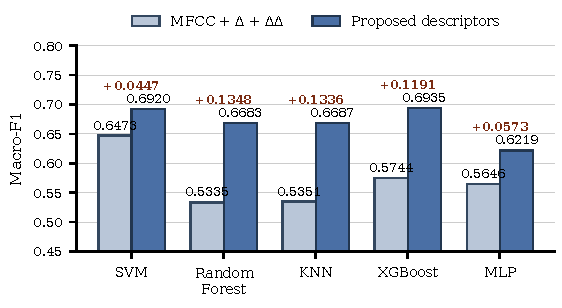
\includegraphics[width=0.70\textwidth]{fig2_features_vs_mfcc.pdf}
\caption{Macro-F1 of the proposed acoustic descriptors and of the MFCC $+$
delta $+$ delta-delta baseline for each classifier; annotations give the
absolute gain of the proposed representation.}
\label{fig:mfcc}
\end{figure}

\subsection{Per-Class Behaviour, Confusion and Discriminability}

Per-class results differ sharply (Fig.~\ref{fig:perclass}). Idgham bi-Ghunnah
is recognised almost perfectly by every classifier (recall $\approx$1.00,
ROC-AUC 1.00), and Qalqalah Wusta remains strong and architecturally stable
across all five models (recall 0.88--0.92, ROC-AUC 0.99). Qalqalah Mushaddadah
is intermediate (recall 0.58--0.72, ROC-AUC 0.89) and Qalqalah Sughra is
recovered reliably by the strongest model (recall 0.55, ROC-AUC 0.84). Idgham
bila-Ghunnah is the most difficult class, with recall spanning 0.017--0.49
across models and ROC-AUC 0.87 for XGBoost; its errors are distributed across
several competitors rather than concentrated in one, indicating overlap with
multiple categories under the current representation. SVM's relatively high
recall for Idgham bila-Ghunnah (0.49) explains its leading balanced accuracy
despite XGBoost's higher Macro-F1. PR analysis shows precision for Idgham
bila-Ghunnah falling steeply as recall increases, so its ROC-AUC must not be
read as uniform strength: the class is ranked above chance, yet only part of it
can be recovered without admitting many false positives.

\begin{figure}[t]
\centering
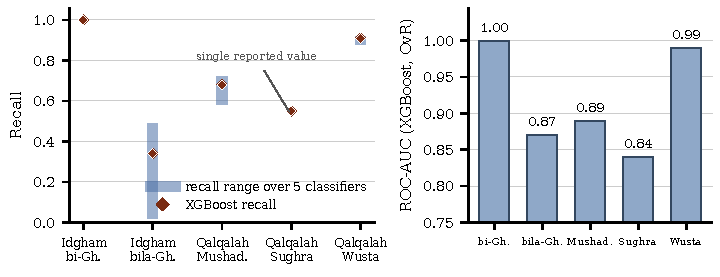
\includegraphics[width=\textwidth]{fig3_perclass.pdf}
\caption{Per-class discriminability of the five Tajweed categories, with the
Idgham subtypes followed by the Qalqalah subtypes. Left: recall attained by the
five classifiers, shown as the range across models with the XGBoost value
marked; Qalqalah Sughra carries a single reported value. Right: ROC-AUC of
XGBoost for the same classes.}
\label{fig:perclass}
\end{figure}

\subsection{Feature Importance and Ablation}

In XGBoost, duration dominates feature importance ($\approx$0.52) followed by
the depth metric ($\approx$0.21); in random forest the same two descriptors lead
(depth $\approx$0.33, duration $\approx$0.24) over a broader distribution.
Ablation confirms their causal contribution (Fig.~\ref{fig:ablation}): removing
the depth metric reduces Macro-F1 from 0.6935 to 0.5169 ($-0.1766$) and removing
duration to 0.5587 ($-0.1348$), whereas retaining duration and depth alone still
yields 0.6424 and nasality alone collapses to 0.2290, i.e.\ no better than
random over five classes. Removing the spectral descriptors (centroid and flux)
costs only 0.0423 Macro-F1, and removing the strongly correlated nasality pair
0.0391, so both groups carry information that complements---but does not
duplicate---the temporal descriptors. The full set remains superior to every
subset and every removal variant: the descriptors are not interchangeable, a
small subset carries most of the discriminative signal, and the residual classes
contribute the difference between a good and the best result.

\begin{figure}[t]
\centering
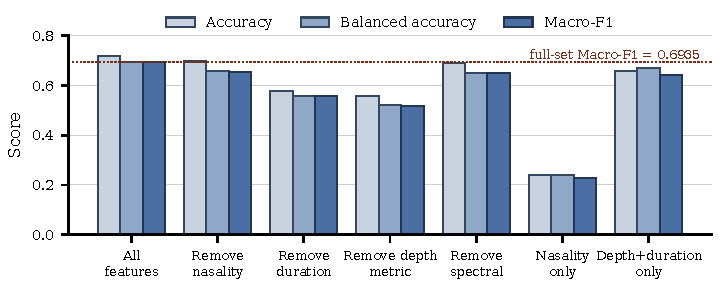
\includegraphics[width=\textwidth]{fig4_ablation.pdf}
\caption{Feature ablation with XGBoost on the held-out test set. Macro-F1,
balanced accuracy and accuracy for seven configurations: the full descriptor
set, four removal variants and two restricted subsets. Protocol, seed and class
weighting are identical throughout.}
\label{fig:ablation}
\end{figure}

\subsubsection{Class-balancing results.}
Balancing trades overall accuracy for minority-class sensitivity
(Fig.~\ref{fig:balancing}). Unbalanced training yields the highest accuracy
(0.7357) but an Idgham bila-Ghunnah recall of only 0.0678 (F1 0.1111). Class
weighting raises that recall to 0.3390 and Macro-F1 to 0.6935 at a cost of 1.55
points of accuracy, and SMOTE gives the strongest balanced performance: balanced
accuracy 0.6617 $\rightarrow$ 0.7121, Macro-F1 0.6592 $\rightarrow$ 0.6951, and
Idgham bila-Ghunnah recall 0.0678 $\rightarrow$ 0.4915 ($+42.4$ points). Borderline-SMOTE is less effective than standard SMOTE, and adding class
weighting after SMOTE yields no further change, indicating that boundary-focused
synthesis does not suit this feature space.

\begin{figure}[t]
\centering
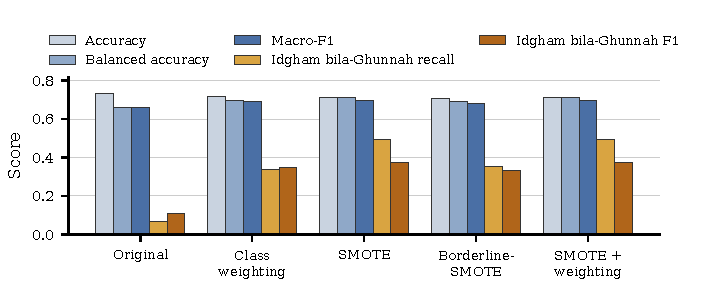
\includegraphics[width=\textwidth]{fig5_balancing.pdf}
\caption{Effect of class-balancing strategies with XGBoost. Accuracy, balanced
accuracy, Macro-F1 and the recall and F1 of the rarest class, Idgham
bila-Ghunnah, for the original training set, class weighting, SMOTE,
borderline-SMOTE and SMOTE combined with class weighting.}
\label{fig:balancing}
\end{figure}

\subsection{Cross-Riwayah Generalisation and Uncertainty}

Training on one riwayah and testing on another yields Macro-F1 between 0.6584
and 0.6718 across the six transfer directions (Fig.~\ref{fig:riwayah}), a narrow
range of 0.0134 with the best transfer Qalun $\rightarrow$ Warsh (0.6718) and
the weakest Qalun $\rightarrow$ Hafs (0.6584): reasonably stable, yet
consistently below the within-distribution XGBoost result, indicating partially
riwayah-independent information alongside residual distribution shift. Bootstrap
resampling gives a mean Macro-F1 of 0.6934 with a 95\% confidence interval of
$[0.6604, 0.7240]$. McNemar (XGBoost vs.\ SVM) and Wilcoxon (original vs.\
SMOTE, 5-fold) tests are specified in the analysis plan but their statistics and
$p$-values are unavailable, so no claim of statistical superiority is
made\todo{insert McNemar and Wilcoxon statistics and p-values}.

\begin{figure}[t]
\centering
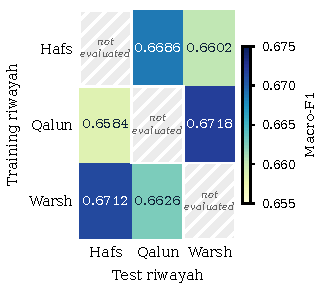
\includegraphics[width=0.40\textwidth]{fig6_cross_riwayah.pdf}
\caption{Cross-riwayah generalisation (Macro-F1): rows are training riwayat and
columns testing riwayat. Diagonal cells (within-riwayah evaluation) correspond
to the pooled results of Table~\ref{tab:models} and are not repeated here.}
\label{fig:riwayah}
\end{figure}


% =====================================================================
\section{Discussion}
\label{sec:discussion}

\subsection{Representation Quality Over Model Complexity}

The results indicate that representation quality, rather than classifier
complexity, primarily determines performance. MFCCs approximate the short-term
spectral envelope and are strong general-purpose descriptors, but Tajweed
realisation depends on temporal organisation, articulatory configuration, nasal
coupling and consonantal release---dimensions that cepstral coefficients encode
only indirectly. That the proposed descriptors improved every classifier, from
instance-based KNN to boosted trees and a neural network, supports the
interpretation that the gain resides in the acoustic evidence itself. The
finding does not establish MFCCs as universally inferior; it shows that, for
this task, a compact linguistically motivated descriptor set carries more
relevant information than the evaluated MFCC configuration, and that model
sophistication cannot compensate for a representation omitting linguistically
relevant dimensions.

\subsection{Duration and Depth as Acoustic Evidence of Tajweed}

Duration and the depth metric converge across two independent forms of
evidence---tree-based importance and controlled removal---making an incidental
explanation unlikely. This is phonetically plausible: assimilation alters the
temporal distribution of energy across a boundary and Qalqalah alters the
release behaviour of a consonant, so both produce measurable temporal and
structural consequences. More broadly, their prominence supports treating
Tajweed as an acoustically observable realisation of phonetic instructions
rather than a purely symbolic property of the text---the premise on which
automatic assessment depends. Because duration is also sensitive to annotation
boundaries (Sect.~\ref{sec:limitations}), its importance should be interpreted
jointly with the boundary-uncertainty analysis.

\subsection{Why Idgham bila-Ghunnah Remains Difficult}

Idgham bi-Ghunnah supplies an explicit nasal cue that nasality descriptors
capture directly, whereas Idgham bila-Ghunnah lacks that marker and must rely on
subtler temporal and spectral assimilation cues that overlap with neighbouring
phonetic events and other target classes. The contrast illustrates the
distinction between phonetic definition and acoustic separability: rules
unambiguous in theory may partially overlap in measured realisation. Scarcity
compounds the problem, and the improvement obtained through SMOTE shows
that part of the difficulty is statistical rather than purely acoustic; residual
confusion after balancing therefore points to genuine acoustic overlap that no
classifier change within the current representation is likely to remove.

\subsection{Generalisation Across Riwayat as Domain Shift}

The stability of cross-riwayah Macro-F1 suggests that the descriptors capture
rule-related information not tied to a single tradition---encouraging for
practical assessment, which must accept recitations in different riwayat. The
consistent degradation relative to within-distribution performance, however,
shows that riwayah-independent classification cannot be assumed: articulation,
timing, melodic realisation and recording conditions shift the feature
distributions of the same category, particularly for duration- and
prosody-sensitive descriptors. Cross-riwayah robustness should therefore be a
design objective, with riwayah-related variability treated as a concrete source
of domain shift for adaptation or invariant-representation methods.

\subsection{Implications for Research and Practice}

Two implications follow. Methodologically, Tajweed recognition should be
modelled as a structured, rule-aware problem: because categories differ in
articulatory mechanism, temporal realisation and acoustic salience, a
representation preserving both shared and rule-specific dimensions is preferable
to a single undifferentiated vector, and domain knowledge remains valuable even
with conventional learners. Practically, interpretable descriptors enable
localised, confidence-aware feedback---a suspected rule occurrence, its temporal
location and the relevant pronunciation dimension---supporting
computer-assisted tutoring beyond global scoring. Such predictions must be
presented as assistive feedback rather than definitive religious or pedagogical
judgement, with expert supervision retained for difficult cases.


% =====================================================================
\section{Limitations}
\label{sec:limitations}

\textbf{Corpus scope.} The corpus covers Juz' 'Amma and two rule families only;
observed characteristics may not represent the wider Qur'an, and fifteen
reciters across three riwayat cannot establish corpus-independent
generalisation, so reported gains are evidence within the experimental domain.
\textbf{Imbalance and synthetic oversampling.} Natural subtype frequencies are
skewed, and SMOTE synthesises feature-space samples rather than authentic
recitations; gains from oversampling partly reflect better feature-space
coverage, not additional phonetic diversity, so class-aware acquisition of
genuine minority examples remains necessary. \textbf{Annotation uncertainty.}
Assimilation phenomena have gradual acoustic transitions, so boundaries are
inherently less discrete; because duration and depth depend on boundary
placement, small shifts can alter feature values for acoustically equivalent
recitations. Quantitative multi-expert agreement analysis and probabilistic
boundaries would strengthen reliability assessment. \textbf{Acoustic
representation.} Segment-level statistics cannot represent long-range
dependencies or transitions between neighbouring phonemes, precisely where
assimilation evidence may reside; sequential or attention-based architectures
should be evaluated alongside---not simply instead of---the interpretable
descriptors. \textbf{External and statistical validity.} Results derive from one corpus and
configuration, so without speaker-independent and external-corpus validation
high in-domain performance does not establish robustness to unseen speakers or
conditions; and without McNemar and Wilcoxon statistics, superiority claims
remain provisional.

\textbf{Future directions.} Three follow-ups address these limits directly.
First, evaluating the identical protocol on the Hafs-only subset of an
independent public recitation corpus would separate corpus-specific from
representation-specific behaviour. Second, a riwayat-conditioned model---with
the reciter's riwayat supplied as an explicit input or with per-riwayat
fine-tuning---should reduce the cross-riwayah penalty without enlarging the
balanced subset. Third, phoneme-aligned rather than fixed-window segmentation
would remove the boundary noise that currently caps the recall of Qalqalah
Mushaddadah and would make the duration descriptor directly interpretable in
terms of Tajweed timing.


% =====================================================================
\section{Conclusion}
\label{sec:conclusion}

This paper formulated automatic Tajweed recognition as a riwayah-aware,
fine-grained acoustic classification problem and instantiated it end to end: a
7{,}998-recording, 11.17\,h corpus of Juz' 'Amma spanning Hafs, Warsh and Qalun;
expert-verified rule-level annotation of Idgham and Qalqalah; an interpretable
eight-descriptor representation; and a five-class evaluation across five
learning paradigms. The representation outperformed an MFCC baseline for every
classifier (best Macro-F1 0.6935, XGBoost), ablation established duration and
the depth metric as dominant cues, balancing materially improved the difficult
Idgham bila-Ghunnah class, and cross-riwayah transfer remained within
0.6584--0.6718. Future work will expand the corpus in surahs, reciters, riwayat
and rules; quantify annotation agreement; adopt speaker- and corpus-independent
evaluation; and investigate sequential, attention-based and multimodal models
combining acoustic evidence with textual and phonological constraints, towards
interpretable, confidence-aware recitation support that complements expert
instruction.


% =====================================================================
\section*{References}
\label{sec:references}

\bibliographystyle{splncs04}
\bibliography{refs}

\end{document}
